\documentclass[12pt,a4paper,oneside]{book} 

%%%%%%%%%%%%%%%%%%%%%%%%%%%%%%%%%%%%%%%%%%%%%%%%%%%%%%%%%%%%%%%%%%%%%%%%

\usepackage{ifthen}
\usepackage{graphicx}
\usepackage[dvips]{epsfig}
\usepackage{enumerate}
\usepackage{calc}
\usepackage{multicol} 
\usepackage{titlesec}
%\usepackage{showkeys}

%%%%%%%%%%%%%%%%%%%%%%%%%%%%%%%%%%%%%%%%%%%%%%%%%%%%%%%%%%%%%%%%%%%%%%%%

\usepackage{a4}
\usepackage{amsfonts}
\usepackage{amssymb}
\usepackage{epsfig}

%%%%%%%%%%%%%%%%%%%%%%%%%%%%%%%%%%%%%%%%%%%%%%%%%%%%%%%%%%%%%%%%%%%%%%%%

\usepackage{t1enc,times}
\usepackage{latexsym,amssymb}
\usepackage{amsmath}
\usepackage{amstext}
%\usepackage[T1]{fontenc}
%\usepackage{cmbright}
\usepackage{pifont}
\usepackage{marvosym}
%\usepackage{pslatex}
% \usepackage{stmaryrd} %=== > dont have it installed on system, doesnt look like it's a compulsory package anyway
%\usepackage{txfonts}  

%%%%%%%%%%%%%%%%%%%%%%%%%%%%%%%%%%%%%%%%%%%%%%%%%%%%%%%%%%%%%%%%%%%%%%%%%%%%%%%

\usepackage[titletoc]{appendix}
\usepackage{mathrsfs}

%%%%%%%%%%%%%%%%%%%%%%%%%%%%%%%%%%%%%%%%%%%%%%%%%%%%%%%%%%%%%%%%%%%%%%%%%%%%%%%

\usepackage{fancybox} 
\usepackage{fancyhdr}
\usepackage{fullpage}

%%%%%%%%%%%%%%%%%%%%%%%%%%%%%%%%%%%%%%%%%%%%%%%%%%%%%%%%%%%%%%%%%%%%%%%%%%%%%%%

%\usepackage{url}    
%\ExecuteOptions{dvips}
%\usepackage[pdftex,colorlinks=true]{hyperref}
%\hypersetup{backref,pdfpagemode=UseThumbs,pdfstartview=Fit,
%pdfpagelayout=SinglePage,pdfstartpage=1,colorlinks=true,menucolor=msc,
%anchorcolor=msc,pagecolor=msc,urlcolor=rfr,breaklinks=true,hyperfootnotes=true}

%%%%%%%%%%%%%%%%%%%%%%%%%%%%%%%%%%%%%%%%%%%%%%%%%%%%%%%%%%%%%%%%%%%%%%%%%%%%%%%

\pagestyle{fancy}
\fancyhf{} 
%\renewcommand{\headrulewidth}{1pt}
%\renewcommand{\footrulewidth}{1pt}
\renewcommand{\headwidth}{\textwidth}
\fancyhead[LE]{\leftmark}
\fancyhead[RO]{\small \rightmark}
\fancyfoot[C]{\thepage}

%%%%%%%%%%%%%%%%%%%%%%%%%%%%%%%%%%%%%%%%%%%%%%%%%%%%%%%%%%%%%%%%%%%%%%%%%%%%%%%

\tolerance 4000
\textwidth 17.00cm
\topmargin -0.30cm
\oddsidemargin -0.25cm
\evensidemargin -0.25cm
\textheight 23.00cm
%\headsep 12pt
\headheight 15pt
\footskip 60pt
%\parindent 12pt

%%%%%%%%%%%%%%%%%%%%%%%%%%%%%%%%%%%%%%%%%%%%%%%%%%%%%%%%%%%%%%%%%%%%%%%%%%%%%%%

\renewcommand{\rmdefault}{ptm}  % times
\renewcommand{\rmdefault}{phv}  % helvetica
\renewcommand{\rmdefault}{pbk}  % bookman
\renewcommand{\rmdefault}{ppl}  % palatino
\renewcommand{\sfdefault}{phv}  % helvetica as sans serif
\renewcommand{\ttdefault}{pcr}  % courier as fixed width
\renewcommand{\tabcolsep}{8pt}
\renewcommand{\arraystretch}{1.25}

%%%%%%%%%%%%%%%%%%%%%%%%%%%%%%%%%%%%%%%%%%%%%%%%%%%%%%%%%%%%%%%%%%%%%%%%%%%%%%%

\newcommand{\Lim}[1]{\raisebox{0.5ex}{\scalebox{0.8}{$\displaystyle \lim_{#1}\;$}}}

%%%%%%%%%%%%%%%%%%%%%%%%%%%%%%%%%%%%%%%%%%%%%%%%%%%%%%%%%%%%%%%%%%%%%%%%%%%%%%%

\def\nn{\nonumber}
\def\f{{\frac}}
\def\pa{{\partial}}
\def\d{{\rm d}}
\def\l{\left}
\def\r{\right}
\def\Mpl{M_{_{\rm Pl}}}

%%%%%%%%%%%%%%%%%%%%%%%%%%%%%%%%%%%%%%%%%%%%%%%%%%%%%%%%%%%%%%%%%%%%%%%%%%%%%%%

\def\done{\marginpar {\scriptsize DONE}}
\def\check{\marginpar {\scriptsize CHECK}}

%%%%%%%%%%%%%%%%%%%%%%%%%%%%%%%%%%%%%%%%%%%%%%%%%%%%%%%%%%%%%%%%%%%%%%%%%%%%%%%

\begin{document}

%%%%%%%%%%%%%%%%%%%%%%%%%%%%%%%%%%%%%%%%%%%%%%%%%%%%%%%%%%%%%%%%%%%%%%%%%%%%%%%

\baselineskip 20pt

%%%%%%%%%%%%%%%%%%%%%%%%%%%%%%%%%%%%%%%%%%%%%%%%%%%%%%%%%%%%%%%%%%%%%%%%%%%%%%%

\pagenumbering{roman}

%%%%%%%%%%%%%%%%%%%%%%%%%%%%%%%%%%%%%%%%%%%%%%%%%%%%%%%%%%%%%%%%%%%%%%%%%%%%%%%

\thispagestyle{empty}
\topskip 15pt
\hrule\hrule\hrule\hrule\hrule
\vskip 20pt
\centerline{\Huge \bf Generation of gravitational waves} 
\vskip 15pt
\centerline{\Huge \bf during inflation} 
\vskip 20pt
\hrule\hrule\hrule\hrule\hrule
\vskip 30pt
\centerline{\Large A project report}
\vskip 8pt
\centerline{\Large submitted in partial fulfilment 
for the award of the degree of}
\vskip 8pt
\centerline{\Large B.S \& M.S in Physics}
%\vskip 8pt
%\centerline{\Large in}
%\vskip 8pt 
%\centerline{\Large Physics}
\vskip 8pt
\centerline{\Large by}
\vskip 8pt
\centerline{\Large \bf Poruri Sai Rahul}
\vskip 8pt
\centerline{\Large under the guidance of}
\vskip 8pt
\centerline{\Large  Dr.~L.~Sriramkumar}
\vskip 30pt 
\begin{center}

\epsfig{file=iitm.eps, width=3.0cm, height=3.0cm} % needed to convert .ps ext to .eps ext.
\end{center}
\vskip 8pt 
\centerline{\Large \bf Department of Physics}
\vskip 8pt 
\centerline{\Large \bf Indian Institute of Technology Madras}
\vskip 8pt 
\centerline{\Large \bf Chennai~600036, India}
\vskip 8pt
\centerline{\Large \bf June~2015}
%%%%%%%%%%%%%%%%%%%%%%%%%%%%%%%%%%%%%%%%%%%%%%%%%%%%%%%%%%%%%%%%%%%%%%%%%%%%%%%

\newpage\topskip 40pt
\centerline{\Large CERTIFICATE}
\thispagestyle{empty}
\vskip 20pt\noindent 
This is to certify that the project titled {\bf Generation of gravitational waves during inflation} is a bona fide record of work done by 
{\bf Poruri Sai Rahul} towards the partial fulfilment of the requirements of the B.S \& M.S degree in Physics at the Indian 
Institute of Technology, Madras, Chennai 600036, India.
\vskip 120pt
\hspace{240pt}(L.~Sriramkumar, Project supervisor)

%%%%%%%%%%%%%%%%%%%%%%%%%%%%%%%%%%%%%%%%%%%%%%%%%%%%%%%%%%%%%%%%%%%%%%%%%%%%%%%

\newpage\topskip 40pt
\thispagestyle{empty}
\centerline{\Large ACKNOWLEDGEMENTS}
\vskip 20pt\noindent 

I cannot express in words my gratitude to {\bf Dr. L.~Sriramkumar} for guiding me, regarding my work and my personal life. 
I would also like to thank V.~Sreenath and Debika Choudhury for helping me with my project and for clarifying my doubts.
I would like to thank my family and my friends, especially Shashi Kunwar and Preeti Saryan, who have kept me on my toes 
over the last few years.
 
 %%%%%%%%%%%%%%%%%%%%%%%%%%%%%%%%%%%%%%%%%%%%%%%%%%%%%%%%%%%%%%%%%%%%%%%%%%%%%%%

\newpage\topskip 40pt
\thispagestyle{empty}
\centerline{\Large ABSTRACT}
\vskip 20pt\noindent 

We are currently in an era of precision cosmology. The precision with which anisotropies in the 
Cosmic Microwave Background, CMB for short, are being measured has increased tremendously over 
the years, thanks to the efforts of the Planck and the WMAP missions. The theory of inflation predicts 
the presence of such anisotropies. In this work, I study the generation and evolution of tensor perturbations, 
otherwise referred to as gravitational waves, during inflation. The aim of this project is to construct a 
python code to numerically evaluate the tensor power spectrum for two different models of inflation, 
namely power law inflation and inflation driven by a small field model of potential.

%%%%%%%%%%%%%%%%%%%%%%%%%%%%%%%%%%%%%%%%%%%%%%%%%%%%%%%%%%%%%%%%%%%%%%%%%%%%%%%

\newpage
\thispagestyle{empty}
\tableofcontents
\newpage

%%%%%%%%%%%%%%%%%%%%%%%%%%%%%%%%%%%%%%%%%%%%%%%%%%%%%%%%%%%%%%%%%%%%%%%%%%%%%%%

\newpage
\thispagestyle{empty}
\listoffigures
\newpage

%%%%%%%%%%%%%%%%%%%%%%%%%%%%%%%%%%%%%%%%%%%%%%%%%%%%%%%%%%%%%%%%%%%%%%%%%%%%%%%

\pagenumbering{arabic}

%%%%%%%%%%%%%%%%%%%%%%%%%%%%%%%%%%%%%%%%%%%%%%%%%%%%%%%%%%%%%%%%%%%%%%%%%%%%%%%

\chapter{Introduction}

\noindent Inflation refers to a period of rapid expansion during the early stages of the radiation dominated epoch of our universe. 
Inflation solves two of the biggest drawbacks of the Hot big bang model namely the horizon problem and the flatness problem. (For a 
detailed review of the horizon problem see Ref.~\cite{Sriramkumar L - 2009}.)

\paragraph*{} This work presents a study of the generation and evolution of tensor perturbations and the power 
spectrum of tensor perturbations generated during two models of inflation, namely power law inflation and inflation
driven by a small field potential model. In this chapter, I shall describe the 
need for scalar fields and the conditions imposed upon them to drive inflation. I shall briefly discuss linear perturbation 
theory and discuss tensor perturbations in the metric. In the next chapter, I shall outline how given a form of the scale 
factor $a(t)$ we can arrive at the dependence of the scalar field $\phi$ and the potential $V(\phi)$ with respect to 
cosmic time $t$. After solving the background equations, I shall discuss the solution to the equation governing tensor 
perturbations and the power spectrum of the tensor perturbations. Finally, I shall discuss the numerical solutions we 
obtained for the power spectrum of tensor perturbations for the two aforementioned models of inflation.

\section{Conventions and notations}

\paragraph*{} Before we go any further, I shall list the conventions and notations adopted in this work. I shall work in $(3+1)-$ dimensions
and I shall adopt the metric signature $(+,-,-,-)$. Greek indices denote all spacetime coordinates where as Latin indices, 
other than $k$, refer to spatial coordinates. I define the Planck mass as $M_{\rm Pl}=\left(8\pi G\right)^{-1/2}$ 
and for convenience, we shall work in units of $M_{\rm Pl} = 1$.
Cosmic time is denoted as $t$ and an overdot denotes differentiation with respect to cosmic time where as 
the conformal time is denoted as $\eta$ and an overprime denotes differentiation with respect to conformal time. 
The duration of inflation can also be measured in terms of number of e-folds $N$ where $N$ is defined as 

\begin{equation}
N = {\rm ln}\left(\frac{a(t)}{a_0}\right),
\end{equation}

\noindent where $a_0$ is the scale factor when inflation started and $a(t)$ is the scale factor when inflation ends.

\section{Driving inflation}

In order to achieve inflation and solve the horizon problem, it is necessary that

\begin{equation}\label{eq:1}
\ddot{a} > 0.
\end{equation}

\paragraph*{} In a spatially flat, smooth, Friedmann universe, the line element is described by

\begin{equation}
{\rm d}s^2 = {\rm d}t^2 - a^2(t){\rm d}{\bf x}^2 = a^2(\eta)\left({\rm d}\eta^2 - {\rm d}{\bf x}^2\right),
\end{equation}

\noindent and for such a line element, the Einstein's equations can be rewritten as the following two Friedmann equations

\begin{equation}\label{eq:F1}
\left(\frac{\dot{a}}{a}\right)^2 = H^2 = \left(\frac{8\pi G}{3}\right)\rho,
\end{equation}

\begin{equation}\label{eq:F2}
\left(\frac{\ddot{a}}{a}\right) = \dot{H} + H^2= -\left(\frac{4\pi G}{3}\right)(\rho + 3p),
\end{equation}

\noindent where $\rho$ and ${\rm p}$ denote the energy density and pressure of the field driving the expansion 
and $H = \dot{a}/a$ is the Hubble parameter

\paragraph*{} From Eqs. (\ref{eq:1}) and (\ref{eq:F2}), it is straight forward to see that

\begin{equation}
(\rho + 3p) < 0,
\end{equation}

\noindent is a necessary condition for the field that drives inflation. We can check that neither matter, for which $p = 0$, 
nor radiation, for which $p = \rho/3$, satisfies the necessary condition. We can therefore, under the necessary conditions, invoke 
a generic scalar field $\phi$ and a corresponding potential $V(\phi)$ to drive inflation. A scalar field that drives inflation 
is also referred to as an Inflaton.

\paragraph*{} We can write the action for such a scalar field as 

\begin{equation}\label{eq:act}
S[\phi] = \int {\rm d}^4x \sqrt{-g}\left[ \left(\frac{1}{2}\right)\left(\partial^{\lambda}\phi \partial_{\lambda}\phi\right) - V(\phi)\right],
\end{equation}

\noindent and the stress-energy tensor for the corresponding scalar field is given by

\begin{equation}\label{eq:se}
T^{\mu}_{\nu} = \partial^{\mu}\phi \partial_{\nu}\phi -\delta^{\mu}_{\nu}\left[\left(\frac{1}{2}\right)\left(\partial^{\lambda}\phi \partial_{\lambda}\phi\right) - V(\phi)\right],
\end{equation}

\noindent From Eqn. (\ref{eq:act}), we can derive the equations of motion for the scalar field as

\begin{equation}\label{eq:feq}
\ddot{\phi} + 3H\dot{\phi} + V_{\phi} = 0,
\end{equation}

\noindent where $V_{\phi} = {\rm d}V/{\rm d}\phi$.

\section{Metric perturbations}

\paragraph*{} Anisotropies in the CMB are one part in $10^5$ and it can be inferred that they should be much smaller at earlier 
epochs given the expanding nature of our universe. We can therefore study the generation and evolution of such perturbations using 
linear perturbation theory. 

\paragraph*{} According to their behaviour under local rotation of the spatial coordinates on hypersurfaces of constant time, 
the perturbations in a Friedmann background can be classified as scalars, vectors and tensors. Scalar perturbations remain 
invariant under rotations. In fact, scalar perturbations are what are most responsible for the 
anisotropy we see in our universe. Under local rotations, vector and tensor perturbations behave as vectors and tensors 
respectively. Rotational velocity fields generate the vector perturbations and are, therefore, also referred to 
as vorticity modes. Finally, gravitational waves are described by tensor perturbations. 
(For a discussion of cosmological linear perturbations theory, refer to Refs. 
\cite{Sriramkumar L - 2009, Dodelson, Durrer, Riotto, Kinney, Linde, B1, B2, G1, AG}.)
For the scope of this work, I shall restrict myself to tensor perturbations of the metric.

\paragraph*{} The Friedmann line element describes a homogeneous and isotropic universe, which is not a valid assumption 
under the presence of perturbations. We can therefore choose to work in a variety of coordinate systems under the condition 
that they reduce to the standard Friedmann line element in the limit when the perturbations vanish. A gauge refers to a 
particular choice of coordinates and a gauge transformation refers to the transformation from one gauge to another. 
Therefore, we can choose to study the evolution of perturbations in terms of gauge-invariant quantities or work in a 
specific gauge throughout. We shall adopt the latter approach. As such, the tensor perturbations in the metric can be 
represented as 

\begin{equation}\label{tpmetric}
{\rm d}s^2 = {\rm d}t^2 - a^2(t)(\delta_{ij} + h_{ij}){\rm d}x^i{\rm d}x^j,
\end{equation}

\noindent where the tensor perturbations are characterized by a transverse, traceless matrix $h_{ij}$. 

\paragraph*{}  In a similar fashion, we shall classify the sources of said metric perturbations, namely the stress-energy tensor. 
The stress energy tensor, similar to the metric tensor, is a symmetric two tensor. Therefore, perturbations in the stress-energy 
tensor can also be classified as scalar, vector and tensor components. A scalar field driving inflation, the inflaton, is a 
scalar source. Velocity fields with vorticity are vector sources. Having eliminated the scalar and vector contributions, 
anisotropic stresses constitute a tensor source. This is referred to as the decomposition theorem.

\paragraph*{} The perturbed Einstein tensors can be derived from the perturbed metric $\delta g_{\mu\nu}$. 
The Einstein's equations can then relate the perturbed Einstein tensors to the perturbed stress-energy tensor, say, $\delta T_{\mu\nu}$. 
These equations govern the evolution of metric perturbations. The decomposition theorem stated above dictates that the scalar, vector and tensor 
perturbations decouple and can therefore be studied independent of one another. In other words, scalar sources lead to 
scalar perturbations, vector sources lead to vector perturbations and tensor sources lead to tensor perturbations. 

\paragraph*{} Under these assumptions, the perturbed Einstein tensors corresponding to the metric described 
by Eqn. (\ref{tpmetric}) are given by

\begin{equation}
\delta G^0_0 = \delta G^0_i = 0,
\end{equation}

\begin{equation}
\delta G^i_j = -\left(\frac{1}{2}\right)\left(\ddot{h}_{ij} + 3H\dot{h}_{ij} - \frac{1}{a^2}\nabla ^2h_{ij}\right),
\end{equation}

\noindent after imposing the conditions that $h_{ij}$ is a transverse and traceless matrix.

\paragraph*{} Similarly, we can write the perturbed stress-energy tensor as

\begin{equation}
\delta T^0_0 = \delta\rho,
\end{equation}

\begin{equation}
\delta T^0_i = \left(\nabla_i\delta\sigma\right),
\end{equation}

\begin{equation}
\delta T^i_j = -\delta p~\delta^i_j.
\end{equation}

\noindent In the absence of anisotropic stresses i.e if $\delta T^i_j = 0$, we get that

\begin{equation}\label{tp}
\ddot{h} + 3H\dot{h} - \left(\frac{1}{a^2}\right)\nabla ^2h = 0.
\end{equation}

\noindent Eqn. (\ref{tp}) can be rewritten in terms of conformal time $\eta$ as

\begin{equation}\label{tpn}
{h}^{''} + 2{\mathcal{H}}{h}^{'} - \nabla ^2h = 0,
\end{equation}

\noindent where ${\mathcal{H}} = a^{'}/a$.

\section{Quantization of perturbations}

\paragraph*{} In Fourier space, Eqn. (\ref{tpn}) becomes

\begin{equation}\label{tp:fs}
h_k^{''} + 2{\mathcal{H}}h_k^{'} + k^2	h_k = 0.
\end{equation}

\paragraph*{} The homogeneity of the Friedmann background allows us to quantize the tensor perturbations. 
Upon quantization, we can write the tensor perturbations $\hat{h}$ in terms of it's Fourier modes $h_k(\eta)$ as

\begin{equation}\label{eq:quant}
\hat{h}(\eta, {\bf x}) = \int \frac{{\rm d}^3\bf{k}}{(2\pi)^{3/2}} \left[\hat{a_k}h_k(\eta)e^{i\bf{k\cdot x}}+ \hat{a_k}^{\dagger}h_k^{*}(\eta)e^{-i\bf{k\cdot x}}\right] ,
\end{equation}

\noindent where the creation and annihilation operators, $\hat{a_k}$ and $\hat{a_k}^{\dagger}$, follow the standard commutation relations. At the linear order in perturbations that we are working in, the power spectrum of the tensor perturbations can be characterized by the two point function of the quantum field $\hat{h}$. The power spectrum of the tensor perturbations ${\mathcal{P}}_{\rm T}(k)$ and the two point function are related by

\begin{equation}\label{eq:quant2}
\int^{\infty}_0 {\rm d}k ~{\mathcal{P}}_{\rm T}(k) = \int {\rm d}^3{\bf{k}}\int\frac{d^3(\bf{x}-\bf{x'})}{(2\pi)^3}~\langle 0|\hat{h}(\eta,{\bf{x}})\hat{h}(\eta, {\bf{x'}})|0\rangle ~e^{-i{\bf{\left[k \cdot (x-x')\right]}}},
\end{equation}

\noindent where $|0\rangle$ is the vacuum state defined as $\hat{a_{\bf k}}|0\rangle = 0 ~\forall ~{\bf k}$. 
Using Eqs. (\ref{eq:quant}) and (\ref{eq:quant2}), we can obtain the tensor power spectrum as

\begin{equation}\label{eq:tps}
{\mathcal{P}}_{\rm T}(k) = 2 \left(\frac{k^3}{2\pi^2}\right) |h_k|^2,
\end{equation}

\noindent where the factor of 2 is needed to take into account the two states of polarization, $+$ and $\times$, of the gravitational waves.

%%%%%%%%%%%%%%%%%%%%%%%%%%%%%%%%%%%%%%%%%%%%%%%%%%%%%%%%%%%%%%%%%%%%%%%%%%%%%%%

\chapter{Inflationary models}

%%%%%%%%%%%%%%%%%%%%%%%%%%%%%%%%%%%%%%%%%%%%%%%%%%%%%%%%%%%%%%%%%%%%%%%%%%%%%%%

\paragraph*{} As mentioned earlier, neither a matter field nor a radiation field can drive inflation. Therefore, under the 
necessary conditions, we can assume that a scalar field $\phi$ and a potential $V(\phi)$ drive inflation. Numerous models 
for the potential function $V(\phi)$ have been proposed, each capable of driving inflation. Power law inflation, inflation 
driven by a small field potential model, slow-roll inflation and chaotic inflation are a few such examples. We shall discuss the first two in more 
detail later in this chapter. The predictions of these models are quantified in terms of the spectral indices of the power 
spectrum of the scalar and tensor perturbations at super-Hubble scales, namely $n_{\rm S}$ \& $n_{\rm T}$ and the ratio of tensor to scalar 
power spectrum at super-Hubble scales $r$.

\paragraph*{} In this chapter, we shall look at two models of inflation namely power law inflation 
and inflation driven by a small field potential model. For the latter of the two models, it is highly non-trivial to 
solve the background equations analytically. We shall therefore only be able to obtain the analytical solutions 
for power law inflation. Numerical solutions for the background and the tensor power spectrum for the latter model 
are discussed in the next chapter. We shall first solve the equations governing the background. Using the solutions of 
the background equations, we shall solve the equations governing the tensor perturbations and obtain the power spectrum 
of the tensor perturbations.

\paragraph*{} From Eq. (\ref{eq:se}), we can write the individual components of the stress-energy tensor for a scalar field $\phi$ as

\begin{equation}\label{eq:se1}
T^{0}_{0} = \left(\frac{\dot{\phi}^2}{2}\right) +V(\phi) = \rho,
\end{equation}

\begin{equation}\label{eq:se2}
T^{i}_{j} = -\left[\left(\frac{\dot{\phi}^2}{2}\right) - V(\phi)\right]\delta^{i}_{j} = -p\delta^i_j.
\end{equation}

\paragraph*{} Using Eqs. (\ref{eq:se1}) and (\ref{eq:se2}), we can rewrite Eqs. (\ref{eq:F1}) and (\ref{eq:F2}) as

\begin{equation}
 \dot{H} = \frac{-\dot{\phi}^2}{2M_{\rm Pl}^2},
\end{equation}

\begin{equation}\label{eq:Hparam}
H^2 = \left(\frac{1}{3M_{\rm Pl}^2}\right)\left(\frac{\dot{\phi}^2}{2} + V\right).
\end{equation}

\noindent We can now express the scalar field $\phi$ and the potential $V$ in terms of cosmic time ${\rm t}$ as

\begin{equation}
\phi(t)= \sqrt{2}M_{\rm Pl} \int dt \sqrt{-\dot{H}},
\end{equation}

\begin{equation}
V(t) = M_{\rm Pl}^2\left(3H^2 + \dot{H}\right).
\end{equation}

\section{Power law inflation}

\paragraph*{} Assume that the scale factor has a power-law form during inflation, namely

\begin{equation}\label{eq:power}
a(t) = a_0t^q.
\end{equation}

\noindent Eq. (\ref{eq:power}) can be written in terms of conformal time $\eta$ as 

\begin{equation}
a(\eta) = \left(-\mathcal{\bar{H}}\eta\right)^{\left(\gamma+1\right)},
\end{equation}

\noindent where $\mathcal{\bar{H}}$ and $\gamma$ are given by 

\begin{equation}
\mathcal{\bar{H}} = a_0^{1/q}(q-1) ~{\rm ~and}~ \gamma  = -\left(\frac{2q-1}{q-1}\right).
\end{equation}

\paragraph*{} We can see that the scalar field and the potential that drive the inflation have the form

\begin{equation}
\frac{\phi(t)}{M_{\rm Pl}} =\sqrt{\left(2q\right)} ~{\rm ln}\left[\sqrt{\left(\frac{V_0}{(3q-1)q}\right)}\left(\frac{t}{M_{\rm Pl}}\right)\right],
\end{equation}

\begin{equation}
V(\phi) = V_0~\exp\left[-\sqrt{\left(\frac{2}{q}\right)}\left(\frac{\phi}{M_{\rm Pl}}\right)\right].
\end{equation}

\paragraph*{} In terms of e-fold ${\rm N}$, we can rewrite $\phi(t)$ as

\begin{equation}
\frac{\phi(N)}{M_{\rm Pl}} = \sqrt{\left(\frac{2}{q}\right)} N - \sqrt{\left(2q\right)}~{\rm ln}~t_0.
\end{equation}

\noindent where $t_0 = \sqrt{\left((3q-1)q/V_0\right)}$

\paragraph*{} Similarly, we can write the Hubble parameter $H$ in terms of e-fold $N$ as 

\begin{equation}
H(N) = H_0\exp^{-N/q}.
\end{equation}

\noindent We also introduce a new parameter $\epsilon_1(N)$, which is defined as

\begin{equation}
\epsilon_1(N) = \frac{1}{2}\left(\frac{{\rm d}\phi}{{\rm d} N}\right)^2 = \frac{1}{q},
\end{equation}

\paragraph*{} Having solved for the scalar field and the Hubble parameter, we can now attempt to solve the 
equation governing the tensor perturbations. We can rewrite Eq. (\ref{tp}), by substituting $h_k = \left(u_k/a\right)$, as

\begin{equation}\label{eq:MS}
u''_k + \left[k^2 - \left(\frac{a''}{a}\right)\right]u_k = 0,
\end{equation}

\noindent and the power spectrum governing tensor perturbations, namely Eq. (\ref{eq:tps}), becomes
\begin{equation}
{\mathcal{P}}_{\rm T}(k) = 2 \left(\frac{k^3}{2\pi^2}\right) |h_k|^2 = 2 \left(\frac{k^3}{2\pi^2}\right) \left(\frac{|u_k|}{a}\right)^2.
\end{equation}

\subsection{The Bunch-Davies initial conditions}

\paragraph*{} In order to arrive at the analytical solutions to the tensor perturbations in fourier space, we need 
to understand the initial conditions from which these perturbations evolved. We impose the initial conditions 
when the modes are well inside the Hubble radius i.e when $\eta \rightarrow -\infty$ or $(k/aH) >> 1$.
In such a sub-Hubble limit,  the curvature of spacetime can be neglected.
Further, upon imposing the condition that $u_k$ are positive frequency modes,
 we can arrive at the solution to the Eq. (\ref{eq:MS}) in the sub-Hubble limit as

\begin{equation}\label{eq:bd}
\Lim{\left(k/aH\right) \rightarrow \infty} u_k(\eta) \rightarrow \left(\frac{1}{\sqrt{2k}}\right){\rm e}^{-ik\eta}.
\end{equation}

\subsection{Tensor power spectrum}

\paragraph*{} Now that we've obtained the solutions for the background and the initial conditions 
governing the tensor perturbations, we shall attempt to solve the equation governing the tensor perturbations 
and obtain the power spectrum of the tensor perturbations.	 

\paragraph*{} Substituting the scale factor given by Eq. (\ref{eq:power}) in the Eq. (\ref{eq:MS}), we can arrive at a 
solution that satisfies the initial conditions Eq. (\ref{eq:bd}) as 

\begin{equation}
u_k(\eta) = \left(\frac{-\pi\eta}{4}\right)^{1/2}{\rm e}^{i[\nu+(1/2)](\pi/2)}{\rm H}_{\nu}^{(1)}(-k\eta),
\end{equation}

\noindent where $\nu = [\gamma + (1/2)]$ and ${\rm H}_{\nu}^{(1)}$ is the 
Hankel function of the first kind and of order $\nu$ (Ref. \cite{Ab}).

\paragraph*{} In the super-Hubble limit $($ i.e as $(-k\eta \rightarrow 0))$, we can approximate the Hankel function to

\begin{equation}
{\rm H}_{\nu}^{(1)}(z) \sim -(i/\pi)\Gamma(\nu)\left(\frac{z}{2}\right)^{(-\nu)}.
\end{equation}

\noindent where $\Gamma(\nu)$ is a Gamma function.

\paragraph*{} In the super-Hubble limit, $u_k$ and the scale factor $a$ have similar behaviour. Therefore, 
the tensor amplitude $h_k$ reaches a constant value and the tensor power spectrum can be written as

\begin{equation}
\mathcal{P}_{\rm T}(k) = A_T\bar{\mathcal{H}}^2\left(\frac{k}{\mathcal{\bar{H}}}\right)^{2(\gamma+2)},
\end{equation}

\noindent where

\begin{equation}
A_T = \left[\frac{1}{\pi^3M_{\rm Pl}^2}\right]\left(\frac{|\Gamma(\nu)|^2}{2^{(2\gamma+1)}}\right).
\end{equation}

\paragraph*{} In this case, the spectral index of the tensor power spectrum in the super-Hubble limit is 

\begin{equation}
n_T = 2(\gamma+2) = \frac{-2}{q-1}.
\end{equation}

\section{Inflation driven by small field potential}

\paragraph*{} We shall assume that the potential $V(\phi)$ that drives inflation is of the form 

\begin{equation}\label{eq:small}
V = V_0\left[1 - \left(\frac{\phi}{\mu}\right)^p\right],
\end{equation}

\noindent where $p = 4$, $\mu/M_{\rm Pl}= 15$ and $V_0/M_{\rm Pl}^4 = 5.55702\times10^{-10}$.

\paragraph*{} Substituting Eq. (\ref{eq:small}) in Eq. (\ref{eq:feq}) and using the expression for H from the Eq. (\ref{eq:Hparam}), we get

\begin{equation}
\ddot{\phi} + \left(\frac{\sqrt{3}}{M_{\rm Pl}}\right)\left(\frac{\dot{\phi}^2}{2} + V\right)\dot{\phi} - \frac{pV_0}{\mu}\left(\frac{\phi}{\mu}\right)^{(p-1)} = 0.
\end{equation}

\paragraph*{} We shall not attempt to obtain an analytical solution for the above expression, instead we solved for $\phi(N)$ numerically. 
Further details regarding the numerical procedure are provided in the next chapter.

%%%%%%%%%%%%%%%%%%%%%%%%%%%%%%%%%%%%%%%%%%%%%%%%%%%%%%%%%%%%%%%%%%%%%%%%%%%%%%%

\chapter{Numerical results}

\paragraph{} In this section, I describe the procedure adopted to numerically evaluate the tensor power spectrum of gravitational waves in a power-law inflationary scenario and in a scenario where inflation is driven by a small-field potential model. Note that we are working in units of $M_{\rm Pl} = 1$.

\section{Power-law inflation}

\paragraph{} Assuming an inflationary potential $V(\phi)$ of the form

\begin{equation}
V(\phi) = V_0 \exp\left[-\sqrt{\frac{2}{q}}\left(\phi - \phi_i\right)\right],
\end{equation}

\noindent where $\phi$ represents the scalar field driving inflation, $\phi_i$ is the initial value at $N=0$ and $q$ is the power-law index.

\paragraph*{} Eqn (\ref{eq:feq}) can be written in terms of e-fold time $N$ as

\begin{equation}\label{eq:temp}
\frac{{\rm d}^2\phi}{{\rm d}N^2} + \left[3 - \frac{1}{2}\left(\frac{{\rm d}\phi}{{\rm d}N}\right)^2\right]\frac{{\rm d}\phi}{{\rm d}N} + \left[6 - \left(\frac{{\rm d}\phi}{{\rm d}N}\right)^2\right]\frac{1}{2V(\phi)}\frac{{\rm d}V(\phi)}{{\rm d}N} = 0.
\end{equation}

\noindent Note that I have made used of the following definition for H to arrive at the above expression

\begin{equation}
H^2 = \frac{2V(\phi)}{3-({\rm d}\phi/{\rm d}N)^2}.
\end{equation}

\paragraph*{} We numerically integrate the Eq.(\ref{eq:temp}) using a 
fourth-order Runge-Kutta method, implemented in Python (Refs. \cite{python, numpy, matplotlib}). Integration was performed from 
e-fold time $N = 0$ to $N = 70$ while assuming the initial conditions for $\phi$ and 
${\rm d}\phi/{\rm d}N$ at $N = 0$ to be 

\begin{equation}
\frac{\phi}{M_{\rm Pl}} = 1,
\end{equation}

\noindent and

\begin{equation}
\frac{{\rm d}\phi}{{\rm d}N} = \left(\frac{\sqrt{2q}}{t_0}\frac{1}{H_0}\right)M_{\rm Pl},
\end{equation}

\noindent where $H_0$ is the value of the Hubble parameter at $N=0$.

\paragraph*{} Figures \ref{field_p}, \ref{Hubble_p} and \ref{epsilon_p} show the theoretical and 
numerical estimate of $\phi$, $H$ and $\epsilon_1$ as a function of $N$. As can be seen, the 
theoretical and numerical estimates are in good agreement with one another.

\begin{figure}
\begin{center}
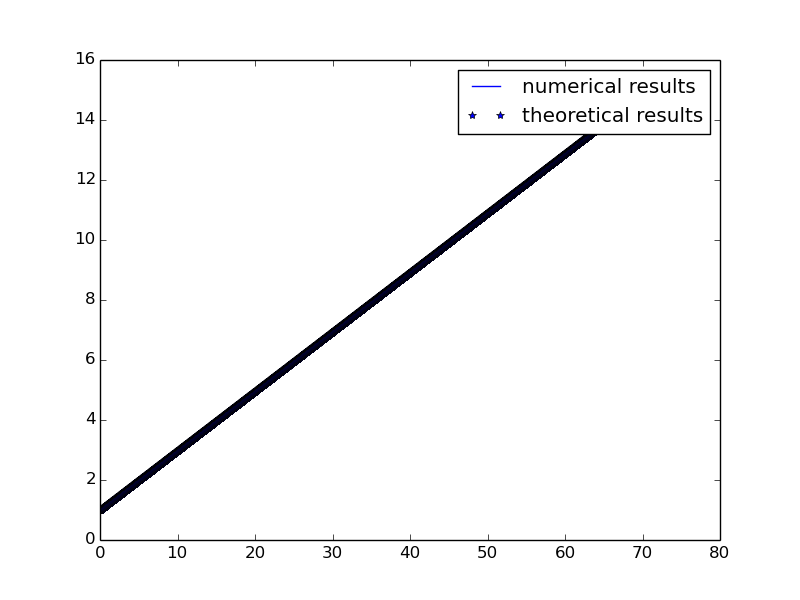
\includegraphics[scale=0.6]{plots/phi_vs_N_power_law.png}
\caption[Plot of $\phi(N)$ as a function of $N$ during power law inflation]{Plot of $\phi(N)$ as a function of $N$ during power law inflation}
\label{field_p}
\end{center}
\end{figure}

\begin{figure}
\begin{center}
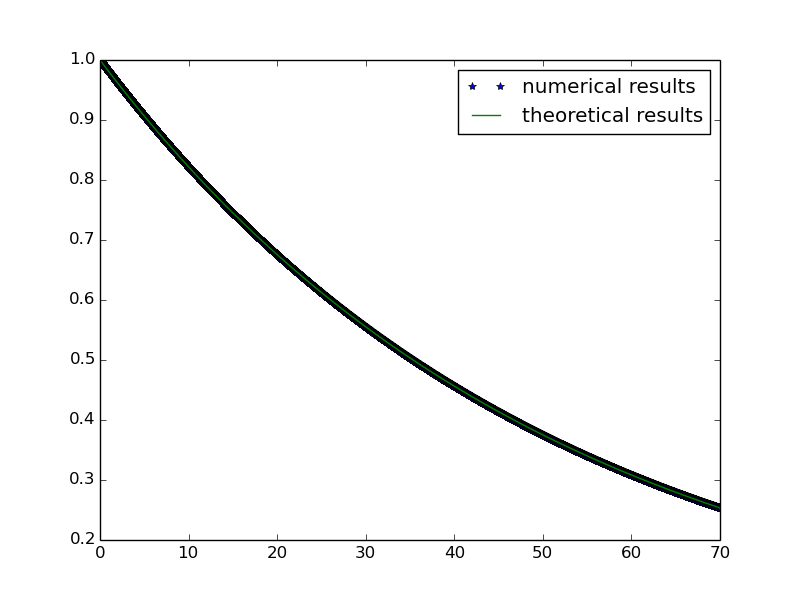
\includegraphics[scale=0.6]{plots/H_vs_N_power_law.png}
\caption[Plot of $H(N)$ as a function of $N$ during power law inflation]{Plot of $H(N)$ as a function of $N$ during power law inflation}
\label{Hubble_p}
\end{center}
\end{figure}

\begin{figure}
\begin{center}
\includegraphics[scale=0.6]{plots/eps_vs_N_power_law.png}
\caption[Plot of $\epsilon_1(N)$ as a function of $N$ during power law inflation]{Plot of $\epsilon_1(N)$ as a function of $N$ during power law inflation}
\label{epsilon_p}
\end{center}
\end{figure}

\paragraph*{} Using the numerical solutions to the background, namely $\phi(N)$ and $H(N)$, we can now solve the equation 
governing the tensor perturbations. Rewriting the Eq. (\ref{tp:fs}) in terms of e-fold time, we arrive at

\begin{equation}\label{eq:temp2}
\frac{{\rm d}^2h_k}{{\rm d}N^2} +\left (3+\frac{1}{H}\frac{{\rm d}H}{{\rm d}N}\right)\frac{{\rm d}h_k}{{\rm d}N} + \frac{k^2}{a^2H^2}h_k = 0.
\end{equation}

\paragraph*{} The above equation was numerically integrated using a fourth order Runge-Kutta method, implemented in Python. 
It is to be noted that $h_k$ was numerically evaluated for various values of $k$, ranging from $10^{-6}$ to $10^{0}$ ${\rm Mpc}^{-1}$. 
For each value of $k$, the initial and final limits of integration in terms of e-fold $N$ were calculated by solving for $N$ when the 
modes are well inside the Hubble scale $(k/aH =  100)$ and when the modes are well outside the Hubble scale $(k/aH =  10^{-5})$. 
Using Eq. (\ref{eq:bd}), the initial values for $h_k$ and ${\rm d}h_k/{\rm d}N$ were set to be

\begin{equation}
h_k  = \frac{1}{\sqrt{2k_0}a(N)},
\end{equation}

\begin{equation}
\frac{{\rm d}h_k}{{\rm d}N} = -\frac{1}{\sqrt{2k_0}a(N)} - \frac{i\sqrt{(k_0/2)}}{a^2(N)H(N)},
\end{equation}

\paragraph*{} Now that we have successfully obtained a numerical solution for $h_k$, 
we can evaluate the tensor power spectrum using Eq. (\ref{eq:tps}). Figure \ref{tps_p} 
shows the numerical estimate of $\mathcal{P}_{\rm T}(k)$ as a function of $k$.

\begin{figure}
\begin{center}
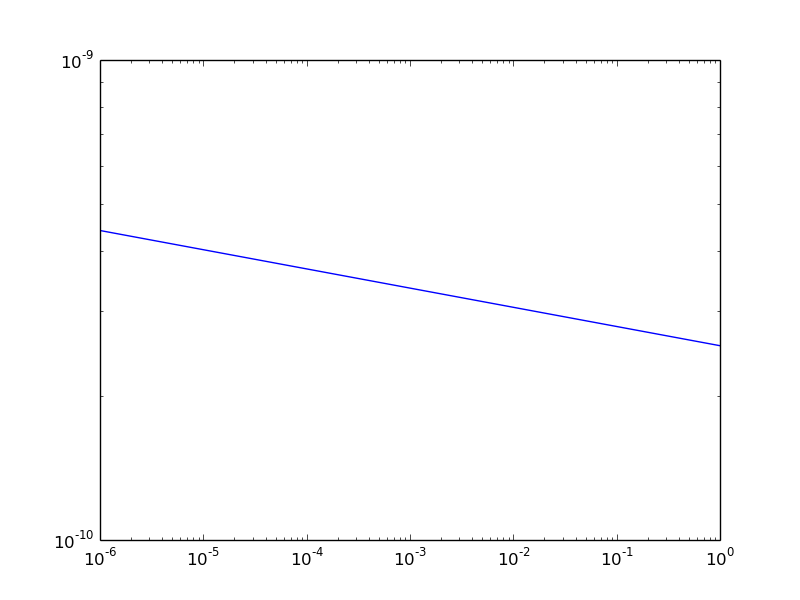
\includegraphics[scale=0.6]{plots/power_spectrum_power_law.png}
\caption[Plot of $\mathcal{P}_{\rm T}(k)$ as a function of $k$ during power law inflation]{Plot of $\mathcal{P}_{\rm T}(k)$ as a function of $k$ during power law inflation}
\label{tps_p}
\end{center}
\end{figure}

\section{Inflation driven by a small field potential}

\paragraph*{} For a small field potential model, given by Eq. (\ref{eq:small}), we repeated the above process to estimate the scalar field $\phi$, 
the Hubble parameter $H$, $\epsilon_1$ and the tensor power spectrum $\mathcal{P}_{\rm T}(k)$.

\paragraph*{} To solve the background equation governing the evolution of $\phi$ numerically, we assumed that at
$N = 0$, $\phi/M_{\rm Pl} = 7.3$ and that ${\dot{\phi}}/M_{\rm Pl}^2 = 8\times10^{-7}$.

\begin{figure}
\begin{center}
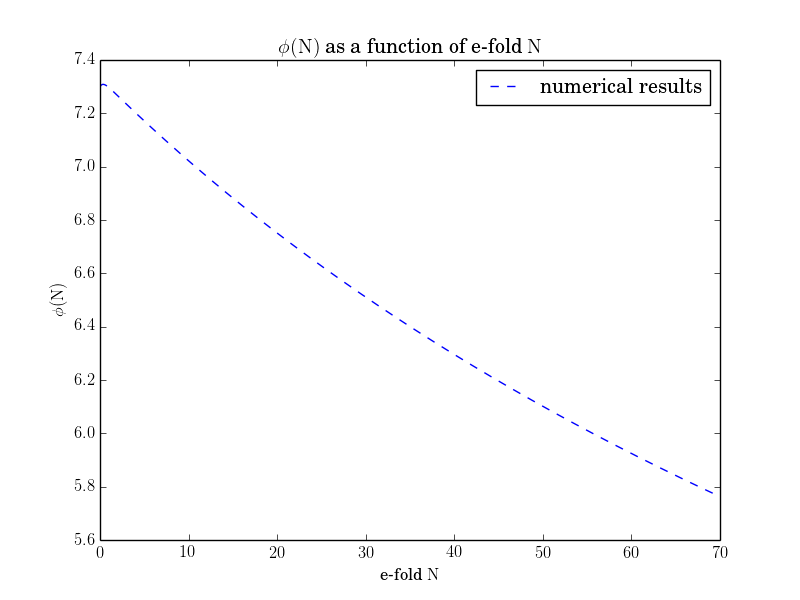
\includegraphics[scale=0.6]{plots/phi_vs_N_small_field.png}
\caption[Plot of $\phi(N)$ as a function of $N$ during inflation driven by a small field potential ]{Plot of $\phi(N)$ as a function of $N$ during inflation driven by a small field potential}
\label{fig:field_sma}
\end{center}
\end{figure}

\begin{figure}
\begin{center}
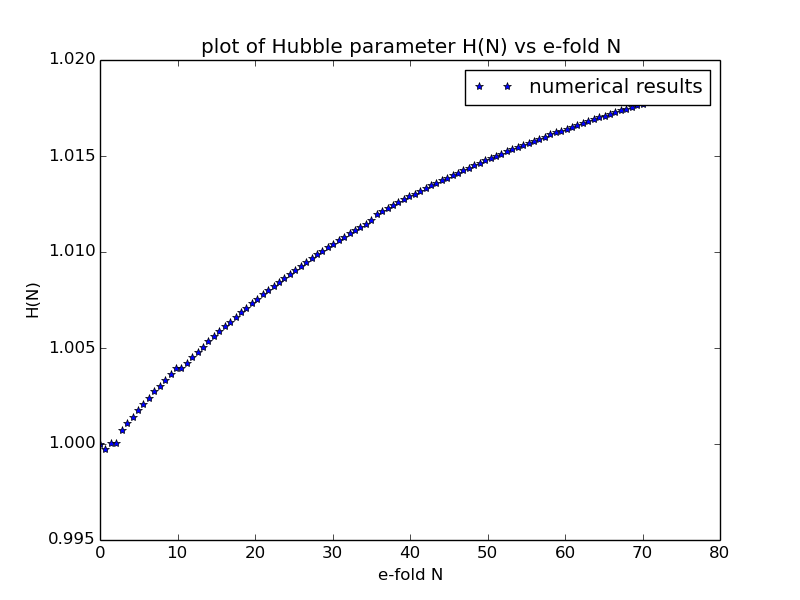
\includegraphics[scale=0.6]{plots/H_vs_N_small_field.png}
\caption[Plot of $H(N)$ as a function of $N$ during inflation driven by a small field potential]{Plot of $H(N)$ as a function of $N$ during inflation driven by a small field potential}
\label{fig:Hubble_sma}
\end{center}
\end{figure}

\begin{figure}
\begin{center}
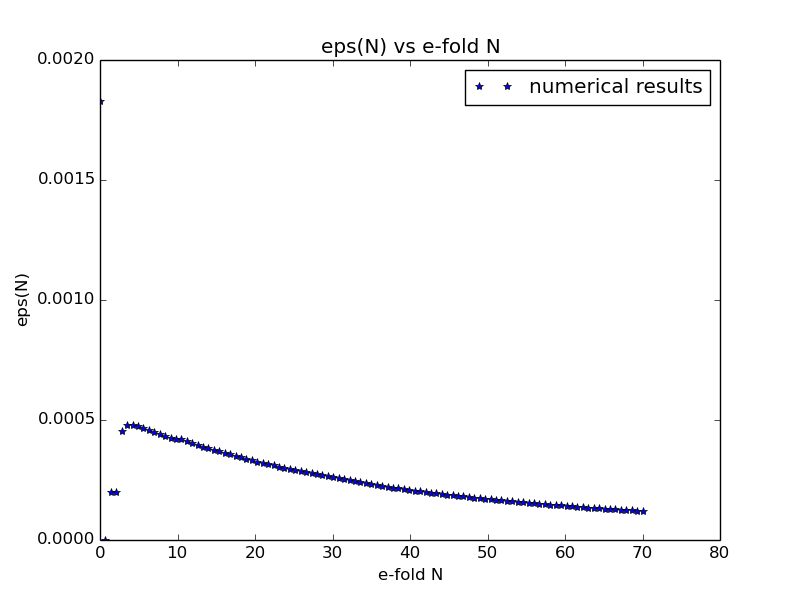
\includegraphics[scale=0.6]{plots/eps1_vs_N_small_field.png}
\caption[Plot of $\epsilon_1(N)$ as a function of $N$ during inflation driven by a small field potential ]{Plot of $\epsilon_1(N)$ as a function of $N$ during inflation driven by a small field potential }
\label{fig:epsilon_sma}
\end{center}
\end{figure}

\begin{figure}
\begin{center}
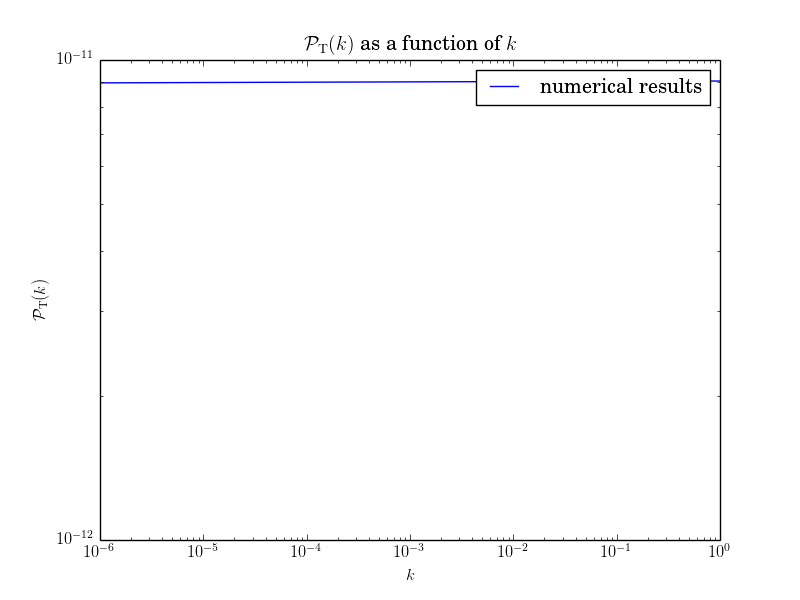
\includegraphics[scale=0.6]{plots/power_spectrum_small_field.png}
\caption[Plot of $\mathcal{P}_{\rm T}(k)$ as a function of $k$ during inflation driven by a small field potential ]{Plot of $\mathcal{P}_{\rm T}(k)$ as a function of $k$ during inflation driven by a small field potential }
\label{fig:tps_sma}
\end{center}
\end{figure}

\paragraph*{} Figures \ref{fig:field_sma}, \ref{fig:Hubble_sma} and \ref{fig:epsilon_sma} show the numerical estimates of 
$\phi$, $H$ and $\epsilon_1$ as a function of $N$. Figure \ref{fig:tps_sma} shows the numerical estimate of 
the tensor power spectrum $\mathcal{P}_{\rm T}(k)$  as a function of $k$ during inflation driven by small field 
model of potential.

%%%%%%%%%%%%%%%%%%%%%%%%%%%%%%%%%%%%%%%%%%%%%%%%%%%%%%%%%%%%%%%%%%%%%%%%%%%%%%%

\chapter{Summary}

\paragraph*{} In this thesis, we have studied tensor perturbations 
in the metric and evaluated the power spectrum of the tensor perturbations. 
We have also numerically estimated the power spectrum of tensor perturbations 
in the super-Hubble limit.

\paragraph*{} In the first chapter, we discussed how neither a matter field nor a radiation field can drive 
inflation and we understood the conditions imposed on a scalar field to drive inflation. We had written down 
the stress-energy tensor corresponding to the scalar field and we arrived at the equation governing the 
evolution of the scalar field. Using the perturbed Einstein tensors and 
the perturbed stress-energy tensor, we were able to arrive at an equation governing the 
evolution of tensor perturbations. We then quantized the tensor perturbations in terms of it's Fourier modes 
and arrived at an analytic form of the power spectrum of tensor perturbations.

\paragraph*{} In the second chapter, we discussed the analytical solutions of the scalar field $\phi$ and 
the potential $V(\phi)$ during power law inflation. After solving the background, we obtained an 
analytic solution to the tensor perturbations and obtained the power spectrum of tensor perturbations 
in the super-Hubble limit. We briefly discuss inflation driven by a small field potential model.

\paragraph*{} In the third chapter, we discussed the methods used to arrive at the numerical solutions 
to the scalar field, the Hubble parameter and $\epsilon_1$ as a function of e-fold $N$ and the tensor 
power spectrum $\mathcal{P}_{\rm T}(k)$ as a function of $k$. 
We studied two forms of the potential, namely power law and small field models 
of the potential. Using a python code, we were able to obtain numerical solutions that were in good agreement with the 
theoretical estimates for power law inflation. We also arrived at the numerical solutions for the small 
field potential model. 

%%%%%%%%%%%%%%%%%%%%%%%%%%%%%%%%%%%%%%%%%%%%%%%%%%%%%%%%%%%%%%%%%%%%%%%%%%%%%%%
\begin{thebibliography}{99}
%%%%%%%%%%%%%%%%%%%%%%%%%%%%%%%%%%%%%%%%%%%%%%%%%%%%%%%%%%%%%%%%%%%%%%%%%%%%%%%

\bibitem{Sriramkumar L - 2009}
L. Sriramkumar, arXiv:0904.4584.

\bibitem{Dodelson}
S. Dodelson, Modern Cosmology (Academic Press, San Diego, 2003).

\bibitem{Durrer}
R. Durrer, Fund. Cosmic Phys. {\bf 15}, 209 (1994).

\bibitem{Riotto}
A. Riotto, arXiv:hep-ph/0210162.

\bibitem{Kinney}
W. H. Kinney, astro-ph/0301448.

\bibitem{Linde}
A. D. Linde, Particle Physics and Inflationary Cosmology (Harwood Academic, Switzerland, 1990).

\bibitem{B1}
R. H. Brandenberger, Rev. Mod. Phys. {\bf 1}, 57 (1985).

\bibitem{B2}
V. F. Mukhanov, H. A. Feldman, and R. H. Brandenberger, Phys. Rep. {\bf 215}, 203 (1992).

\bibitem{G1}
M. Giovannini, Int. J. Mod. Phys. D {\bf 14}, 363 (2005).

\bibitem{AG}
A. Guth, Phys. Rev. D {\bf 23}, 347 (1981).

\bibitem{Ab}
M. Abramowitz and I. A. Stegun, Handbook of Mathematical Functions (Dover Publications, New York, 1964).

\bibitem{python}
Guido van Rossum: Python Reference Manual, CWI Report CS-R9525 (1995).

\bibitem{numpy}
Stefan van der Walt, S. Chris Colbert and Gael Varoquaux, Computing in Science and Engineering {\bf 13}, 22 (2011).

\bibitem{matplotlib}
John D. Hunter, Computing in Science and Engineering {\bf 9}, 90 (2007).

% http://www.scipy.org/citing.html
% http://academia.stackexchange.com/questions/5482/how-do-i-reference-the-python-programming-language-in-a-thesis-or-a-paper
% https://www.python.org/~guido/Publications.html
% http://matplotlib.org/citing.html

%%%%%%%%%%%%%%%%%%%%%%%%%%%%%%%%%%%%%%%%%%%%%%%%%%%%%%%%%%%%%%%%%%%%%%%%%%%%%%%
\end{thebibliography}
%%%%%%%%%%%%%%%%%%%%%%%%%%%%%%%%%%%%%%%%%%%%%%%%%%%%%%%%%%%%%%%%%%%%%%%%%%%%%%%

\begin{appendices}
\chapter{Python Code}

\paragraph*{} We have attached a python code that evaluates the theoretical and numerical estimates for 
the scalar field $\phi$, 
the Hubble parameter $H$, $\epsilon_1$ as a function of e-fold $N$ and the power spectrum of the 
tensor perturbations in the super-Hubble limit ${\mathcal{P}}_{\rm T}(k)$ as a function of $k$ during 
power law inflation. To arrive at the numerical estimates during inflation driven by a small field potential model, 
we shall replace the potential function with Eq. (\ref{eq:small}) and change the relevant constants. 

\paragraph*{} Eq. (\ref{eq:temp}) is solved numerically using a fourth order Runge-Kutta method 
and $H$, $\epsilon_1$ are obtained from the numerical solution of $\phi(N)$. 
After we solve the background, we solve Eq. (\ref{eq:temp2}) numerically using a fourth order Runge-Kutta method. 
Using the numerical solutions for $h_k$ and Eq. (\ref{eq:tps}), we can numerically evaluate the power spectrum. 
Note that we are working in units of $M_{\rm Pl} = 1$

\newpage

\begin{small}
\begin{verbatim}
import numpy
import matplotlib.pyplot as plt

plt.rc('text', usetex=True)
plt.rc('font', family='serif')

tps_file = open('power_spectrum_power_law.dat','w')
phi_file = open('phi_vs_N_power_law.dat','w')
h_file = open('H_vs_N_power_law.dat','w')
eps_file = open('eps1_vs_N_power_law.dat','w')

q = 51.
V0 = (204./100.)*1e-08
t0 = (q*(3.*q -1.)/V0)**(1./2)

phi0 = 1.
dphi0 = (2.*q)**(1./2)/t0

Ni = 0.
Nf = 70. 

kp = 5.*1e-02
beta = -((2.*q -1.)/(q -1.))
eps1a = ((beta +2.)/(beta +1.))

V = lambda phi : V0*numpy.exp(-(2./q)**(1./2)*(phi -phi0))
dV=lambda phi :-(2./q)**(1./2)*V0*numpy.exp(-(2./q)**(1./2)*(phi -phi0))

H0 = ((1./3)*(dphi0**2/2. +V(phi0)))**(1./2.)
Dphi0 = dphi0/H0

def DDphi(N, phi0, Dphi0):
    return -(3 -Dphi0**2/2.)*Dphi0 -(dV(phi0)/(2*V(phi0)))*(6 -Dphi0**2)

def rk4_step(N, phi0, Dphi0, step):
    F1 = Dphi0
    f1 = DDphi(N, phi0, Dphi0)
    F2 = Dphi0 +f1*step/2.
    f2 = DDphi(N +step/2., phi0 +F1*step/2., Dphi0 +f1*step/2.)
    F3 = Dphi0 +f2*step/2.
    f3 = DDphi(N +step/2., phi0 +F2*step/2., Dphi0 +f2*step/2.)
    F4 = Dphi0 +f3*step
    f4 = DDphi(N +step, phi0 +F3*step, Dphi0 +f3*step)  

    return [(f1 +2*f2 +2*f3 +f4)*step/6., 
    		(F1 +2*F2 +2*F3 +F4)*step/6.] # [Dphi, phi] update

npts = 100000
step = (Nf-Ni)/(npts)

phi_ = phi0
Dphi_ = Dphi0

phi_array = numpy.array([phi_])
Dphi_array = numpy.array([Dphi_])
N_array = numpy.array([Ni]) 

phi_theory = lambda N : (2./q)**(1./2)*N + phi0

N = Ni
phi_file.write(str(N)+"\t"+str(phi_)+"\t"
		+str(Dphi_)+"\t"+str(phi_theory(N))+"\n")
while N < Nf:
    array = rk4_step(N, phi_, Dphi_, step)
    phi_ = phi_ + array[1]
    Dphi_ = Dphi_ + array[0]
    phi_array = numpy.append(phi_array,phi_)
    Dphi_array = numpy.append(Dphi_array,Dphi_)
    N += step
    N_array = numpy.append(N_array,N)
    phi_file.write(str(N)+"\t"+str(phi_)+"\t"
    		+str(Dphi_)+"\t"+str(phi_theory(N))+"\n")

phi_file.close()

phi = lambda N : phi_array[int((N-Ni)/step)]
Dphi = lambda N : Dphi_array[int((N-Ni)/step)]

plt.cla()
plt.hold(True)
plt.xlim([Ni,Nf])
plt.xlabel(r'e-fold ${\rm N}$')
plt.ylabel(r'$\phi({\rm N})$')
plt.title(r'$\phi({\rm N})$ as a function of e-fold ${\rm N}$')
numerical, = plt.plot(N_array, phi_array, 
	'--', label = 'numerical results')
theory, = plt.plot(N_array, [phi_theory(N) for N in N_array],
		 '-', label = 'theory results')
plt.legend([numerical, theory], 
		['numerical results', 'theoretical results'])
plt.savefig('phi_vs_N_power_law.png')

eps0 = (3./2)*((dphi0**2)/(dphi0**2/2. + V(phi0)))
eps = 1./q 

H = lambda N : (V(phi(N))/(3 -Dphi(N)**2/2))**(1./2)
DH = lambda N : -(1./2)*H(N)*Dphi(N)**2

H_theory = lambda N : H0*numpy.exp(-N/q)

for N in N_array:
	h_file.write(str(N)+"\t"+str(H(N)/H0)+"\t"+str(H_theory(N)/H0)+"\n")

plt.cla()
plt.hold(True)
plt.xlim([Ni,Nf])
plt.xlabel(r'e-fold ${\rm N}$')
plt.ylabel(r'${\rm H}({\rm N})$')
plt.title(r'${\rm H}({\rm N})$ as a function of e-fold ${\rm N}$')
numerical, = plt.plot(N_array, numpy.asarray([H(i) for i in N_array], 
		dtype= numpy.float64)/H0, '--', label = 'numerical results')
theory, = plt.plot(N_array, [H_theory(N)/H0 for N in N_array], 
		'-', label = 'theory')
plt.legend([numerical, theory], 
		['numerical results', 'theoretical results'])
plt.savefig('H_vs_N_power_law.png')

ai = 1e-05

eps1 = lambda N : Dphi_array[int((N-Ni)/step)]**2/2.
eps1_theory = eps0

for N in N_array:
	eps_file.write(str(N)+"\t"+str(eps1(N))+"\t"+str(eps1_theory)+"\n")

plt.cla()
plt.xlim([Ni,Nf])
plt.xlabel(r'e-fold ${\rm N}$')
plt.ylabel(r'$\epsilon_1({\rm N})$')
plt.title(r'$\epsilon_1({\rm N})$ as a function of e-fold ${\rm N}$')
numerical, = plt.plot(N_array, 
		[str(eps1(i)).strip('[]') for i in N_array], 
		'--', label = 'numerical results')
plt.axhline(y=eps0)
plt.legend([numerical], ['numerical results'])
plt.savefig('eps1_vs_N_power_law.png')

z = lambda N: ai*numpy.exp(N)*Dphi(N)
A = lambda N : ai*numpy.exp(N)

def DDhk(k0, N, hk0, Dhk0):
    return -((3. +(DH(N)/H(N)))*Dhk0 +((k0/(A(N)*H(N)))**2)*hk0)

def rk4_step(k0, N, hk0, Dhk0, step):
    F1 = Dhk0
    f1 = DDhk(k0, N, hk0, Dhk0)
    F2 = Dhk0 +f1*step/2.
    f2 = DDhk(k0, N +step/2., hk0 +F1*step/2., Dhk0 +f1*step/2.)
    F3 = Dhk0 +f2*step/2.
    f3 = DDhk(k0, N +step/2., hk0 +F2*step/2., Dhk0 +f2*step/2.)
    F4 = Dhk0 +f3*step
    f4 = DDhk(k0, N +step, hk0 +F3*step, Dhk0 +f3*step)   

    return numpy.array([(f1 +2*f2 +2*f3 +f4)*step/6.], dtype=complex), 
    		numpy.array([(F1 +2*F2 +2*F3 +F4)*step/6.], dtype=complex) 
    		# [Dhk, hk] update

k_list = numpy.array([10**((-12 + i)/2.) for i in range(13)])
Nics_array = []
Nshs_array = []

for k in k_list:
    Nics_temp = numpy.asarray([k - 1e+02*A(N)*H(N) for N in N_array])
    Nshss_temp = numpy.asarray([k - 1e-05*A(N)*H(N) for N in N_array])
    nics_test = numpy.where(Nics_temp > 0)
    nshss_test = numpy.where(Nshss_temp > 0)
    Nics_array.append(Ni + nics_test[0][-1]*step)
    Nshs_array.append(Ni + nshss_test[0][-1]*step)

Nics_arr = numpy.asarray(Nics_array)
Nshs_arr = numpy.asarray(Nshs_array)

k_min = 1e-6
k_max = 10**(1./2)

k_vs_hk = numpy.zeros(1,dtype=complex)

i = 0
k0 = k_min

while k0 < k_max:
    print 'k0 = ', k0

    Nics = Nics_arr[i]
    Nshss = Nshs_arr[i]

    hk0 = numpy.zeros(1,dtype=complex)
    hk0.real = (((2.*k0)**(1./2))*A(Nics))**(-1.)

    Dhk0 = numpy.zeros(1,dtype=complex)
    Dhk0.real = -(1/A(Nics))*((2*k0)**(-1./2))
    Dhk0.imag = -((k0/2)**(1./2))/(A(Nics)*A(Nics)*H(Nics))
 
    N = Nics
    while N < Nshss:
        array = rk4_step(k0, N, hk0, Dhk0, step)
        hk0 = hk0 + array[1]
        Dhk0 = Dhk0 + array[0]
        N += step

    k_vs_hk = numpy.append(k_vs_hk, hk0) 
    print '\n'
    
    temp = 2*(k0)**3/(2*numpy.pi**2)*(numpy.absolute(hk0))**2
    tps_file.write(str(k0)+"\t"+str(temp).strip('[]')+"\n")
    k0 = 10**(1./2)*k0
    i += 1

k_list = numpy.array([10**((-12 + i)/2.) for i in range(13)])
TPS = [2*(k_list[i])**3/(2*numpy.pi**2)*
		(numpy.absolute(k_vs_hk[i+1]))**2 for i in range(len(k_list))]
print k_list, TPS

tps_file.close()

plt.cla()
plt.xlabel(r'$k$')
plt.ylabel(r'${\mathcal{P}}_{\rm T}(k)$')
plt.title(r'${\mathcal{P}}_{\rm T}(k)$ as a function of $k$')
numerics, = plt.loglog(k_list, TPS)
plt.legend([numerics],['numerical results'])
plt.savefig('power_spectrum_power_law.png')

\end{verbatim}
\end{small}
\end{appendices}
%%%%%%%%%%%%%%%%%%%%%%%%%%%%%%%%%%%%%%%%%%%%%%%%%%%%%%%%%%%%%%%%%%%%%%%%%%%%%%%
\end{document}